% todo: pensar em colocar uma parte falando sobre o método dos mínimos quadrados
\part{Teoria}
	\chapter{Reologia}
		\section{Fundamentos}
		
		% todo: Pensar se eu devo colocar que vem do grego rheos, corrente/rio/fluxo e logia, estudo/ciência
		% todo: pensar se eu devo falar que foi cunhado pelo Prof. Bingham em 1929
		A reologia é a área ciência que estuda o fluxo e a deformação da matéria. Para causar um fluxo ou deformação, é necessário que uma força externa seja aplicada ao corpo. Reagindo à essa força, o material se comporta de tal maneira que algumas de suas características estruturais podem ser inferidas. Isso é feito intuitivamente por qualquer pessoa, por exemplo, ao apertar uma fruta para determinar sua firmeza e assim, se ela está apropriada para consumo ou não, para desagrado do vendedor.  % todo: pensar se eu deixo essa piadinha aqui ou não
		
		No campo coloidal, a reologia é utilizada para estudar como os corpos coloidais estão dispostas no meio, suas interações entre si e com o meio, e como fluem mediante a força externa. Por exemplo, soluções de micelas gigantes são altamente viscosas, pois as cadeias das micelas se entrelaçam e ramificam, então existe um mecanismo para oferecer resistência à força aplicada. Já soluções de micelas esféricas possuem baixa viscosidade, pois o tamanho das micelas é pequeno, e não existe esse mecanismo. A resistência se deve principalmente ao solvente, nesse caso.
		
		A viscosidade pode ser definida, de maneira pouco rigorosa, como a resistência ao fluxo de um material. Então água possui baixa viscosidade, já mel, uma solução concentrada de açúcar, possui alta viscosidade. Porém, quando tenta-se aplicar essa definição para outros tipos de materiais, aparecem problemas. Manteiga mantém seu formato, ao contrário de mel, que sempre flui, mas é muito mais fácil passar manteiga num pedaço de pão do que mel. Qual seria mais viscoso? % todo: mencionar amido de milho funciona?
		
		% todo: checar o tipo de emulsão da manteiga
		O comportamento diferente da manteiga é causado por sua microestrutura coloidal. Manteiga é uma emulsão água em óleo, ou seja, há gotículas de água estabilizadas pelas proteínas do leite dispersas e compactadas num meio contínuo de óleo. As forças atrativas entre as gotículas, e a concentração relativa pequena de óleo, faz com que as gotículas consigam se estruturar no meio, impedindo o fluxo sob uma força externa bastante fraca como a gravidade. Porém, as forças entre as gotículas podem ser rompidas quando uma força externa um pouco mais forte é aplicada. Após o rompimento das interações intergotículas, o fluxo se torna fácil. Se a força for removida, as interações são reformadas e o material volta a assumir sua consistência característica.
		
		Portanto, a viscosidade da manteiga dependeu da força que estava sendo aplicada. Em forças baixas, o material aparentava ser altamente viscoso, já em forças maiores, o material aparentava ser pouco viscoso. Não existe um valor único de viscosidade que pode ser atribuído à manteira, da mesma maneira que é feito com água. Somente é possível estabelecer viscosidades aparentes dependentes da força aplicada.
		
		Do lado oposto à viscosidade, no campo reológico, existe a elasticidade. Materiais elásticos, ao invés de fluir, se deformam reversivelmente. A estrutura interna desses materiais permite que energia seja armazenada em torções e distensões. Quando a força externa é removida, a energia é liberada e o material volta ao seu formato inicial. Caso a energia aplicada supere as forças que estruturam o material, por exemplo, ligações covalentes ou interações intermoleculares, o material acaba fluindo ou quebrando. Exemplos clássicos de materiais elásticos são: molas, borrachas, rochas, madeira. A constante de elasticidade é a grandeza análoga à viscosidade, para materiais elásticos. Essa constante está relacionada à força necessária para causar uma deformação no material.

		Retomando o exemplo anterior, em baixos valores de força, a manteiga conseguia se manter estruturada. Nessa região de forças bastante pequenas, a manteiga consegue armazenar energia em sua estrutura interna. De acordo com as definições apresentadas, a manteiga pode se comportar tanto como um material elástico quanto um material viscoso. Esse tipo de material recebe o nome de material viscoelástico.
		
		\subsection{Número de Deborah}
		
		É possível relacionar materiais viscosos, elásticos e viscoelásticos através do número de Deborah (Eq. \ref{eqn:Deborah}), que relaciona o tempo de relaxação do material (\(\tau_{\text{rel}}\)) com o tempo de observação (\(t\)).
		
		\begin{equation}
			D_e = \dfrac{\tau_{\text{rel}}}{t}
			\label{eqn:Deborah}
		\end{equation}
		
		O tempo de relaxação é, como o nome diz, o tempo que um material leva para dissipar uma tensão aplicada em si. Quando a força é aplicada por um tempo maior que o tempo de relaxação do material, a tensão é dissipada e o material flui. De maneira oposta, caso a tensão seja aplicada por um tempo bastante curto, comparativamente, não há tempo para o material perder a energia, e mantém seu formato.
		
		% todo: achar uma ref pra isso
		Por exemplo, um arco de madeira utilizado para caça ou para guerra devia ser armazenado sem sua corda. Caso fosse, a força do arco cairia com o tempo e a eficácia do arco diminuía. Isso ocorre porque as fibras da madeira que compõe o arco, se tensionadas por muito tempo, conseguem deslizar umas pelas outras para dissipar a tensão. Logo, o arco, notavelmente um material elástico no uso cotidiano, se comporta como um fluido se tensionado por muito tempo.
		
		Água, no outro extremo, é um material que se comporta quase sempre como um líquido. Porém, a água age como um sólido quando um objeto impacta sobre ela, a uma velocidade suficientemente grande. Isso ocorre porque as moléculas de água não tem tempo suficiente para se deslocar, e a água é um fluido incompressível, resultando numa resistência forte ao fluxo.
		
		Soluções de micelas gigantes combinam ambos os comportamentos elástico e viscoso. Isso é observado claramente no efeito de recuo (\emph{recoil}), quando uma solução de micelas gigantes é agitada circularmente. Inicialmente, observa-se a solução seguindo o sentido do fluxo, possivelmente através das bolhas formadas pela agitação. Quando a agitação é cessada, o fluxo continua por um tempo, devido à sua inércia, depois para e começa a fluir no sentido contrário (recuo). As cadeias de micelas gigantes conseguem interagir entre si e se entrelaçar de tal modo que um pouco da energia da agitação é armazenada. Quando a agitação cessa, essa energia consegue ser liberada, o que ocorre no sentido oposto à agitação, então o recuo é observado. Depois do recuo, a solução para de se movimentar pois toda a energia foi dissipada. A escala de tempo para a perda de energia e para o \emph{recoil} são aproximadamente iguais, logo o número de Deborah desse fluido é próximo de 1.
		
		A correlação entre o número de Deborah e o comportamento do material pode ser resumido pela Eq. \ref{eqn:Deborah_casos}
		
		\begin{equation}
			D_e
			\begin{cases}
				\gg 1     & \textrm{Elástico}      \\
				\approx 1 & \textrm{Viscoelástico} \\
				\ll 1     & \textrm{Viscoso}
			\end{cases}
			\label{eqn:Deborah_casos}
		\end{equation}
		
		O arco, em uso, possui \(D_e\gg1\), pois seu tempo de relaxação é bastante longo comparado com a ação de atirar uma flecha, mas \(D_e\ll1\) quando armazenado, o que pode durar meses. Dessa maneira, o arco e os outros materiais citados se comportam como materiais tanto elásticos quanto viscosos, dependendo do tempo de análise \(t\). O nome desse número vem de uma passagem bíblica, \emph{Os montes deslizaram diante do senhor} (Juízes 5:5). Mesmo as montanhas, que tradicionalmente não se movem, acabam deslizando mediante tempos de observação infinitos.
		
		Para um estudo mais aprofundado de reologia, é necessário estabelecer um formalismo matemático, que será feito nas seções a seguir. Primeiramente se
		
			\subsection{Cisalhamento e curvas de fluxo}
			
			O cisalhamento é um tipo de movimento que ocorre no sentido do plano da amostra, perpendicular ao plano normal. A magnitude do cisalhamento \(\gamma\) é calculada a partir da altura \(z\) da amostra e o grau de deformação \(\Delta x\), como mostra a Eq. \ref{eqn:cisalhamento}. \(\gamma\) é adimensional.
			
			\begin{equation}  % todo: pensar em colocar isso em paralelo à uma figura semelhante à da Wikipedia
				\gamma = \frac{\Delta x}{z}
				\label{eqn:cisalhamento}
			\end{equation}
			
			A tensão de cisalhamento \(\tau\) é a força necessária para aplicar um cisalhamento divido pela área de aplicação (Eq. \ref{eqn:tensao_cisalhamento}). A unidade usual para \(\tau\) é Pa.
			
			\begin{equation}
				\tau = \frac{F}{A}
				\label{eqn:tensao_cisalhamento}
			\end{equation}
			
			A velocidade de cisalhamento é conhecida também como taxa de cisalhamento \(\dot{\gamma}\), calculada a partir da derivada em função do tempo de \(\gamma\) (Eq. \ref{eqn:taxa_cisalhamento}). A unidade usual de \(\dot{\gamma}\) é Pa.s\menosUm.
			
			\begin{equation}
				\dot{\gamma} = \dfrac{\delta y}{\delta t}
				\label{eqn:taxa_cisalhamento}
			\end{equation}
			
			É possível obter o valor de viscosidade de um material aplicando-se uma taxa de cisalhamento crescente e medindo a tensão necessária para manter essa taxa (modo \emph{control rate}, \emph{CR}), ou aplicando-se uma tensão e medindo-se a taxa (modo \emph{control stress}, \emph{CS}). A informação resultante desse tipo de análise se chama curva de fluxo.
						
			\subsection{Fluidos Newtonianos}
			
			Os fluidos Newtonianos são caracterizados por possuírem somente um valor para viscosidade \(\eta\), independente da taxa de cisalhamento, relação simbolizada pela Eq. \ref{eqn:Newton}. Um modelo físico frequentemente utilizado para fluidos Newtonianos é o dissipador viscoso (\emph{dashpot}).
			
			\begin{equation}
				\tau = \eta\dot{\gamma}
				\label{eqn:Newton}
			\end{equation}
			
			A figura \ref{fig:reol_newt_exemplos} mostra curvas de fluxo simuladas para um fluido Newtoniano de viscosidade \(\eta=10\:Pa.s^{-1}\).
			
			\begin{figure}[H]
				\begin{subfigure}[t]{.5\textwidth}
					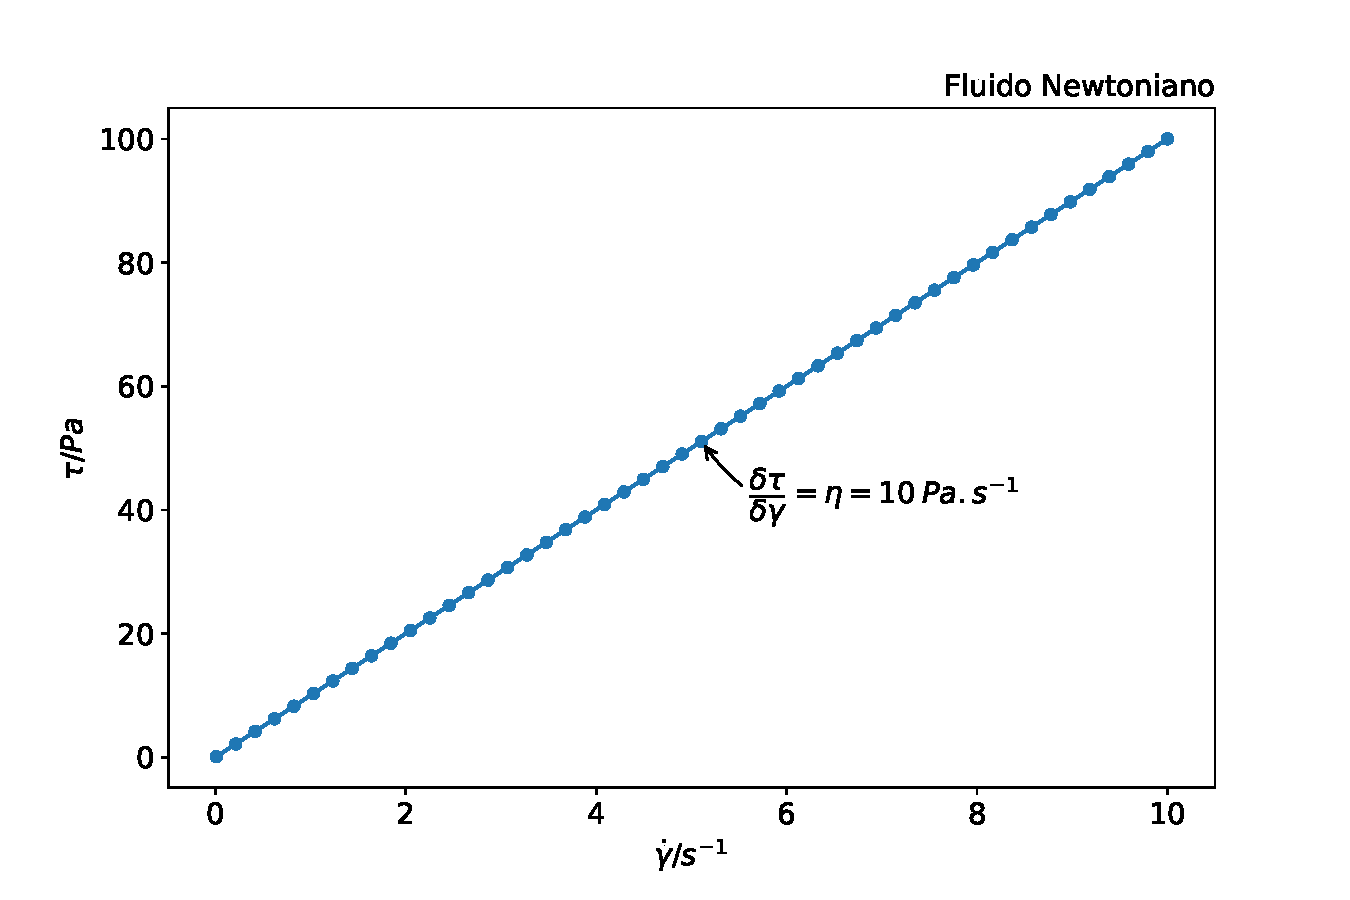
\includegraphics[width=\textwidth]{./imagens/reologia/newtoniano_exemplo_tauGP}
					\caption{\(\tau \times \dot{\gamma}\)}
					\label{fig:reol_newt_tauGP}
				\end{subfigure}%
				\begin{subfigure}[t]{.5\textwidth}
					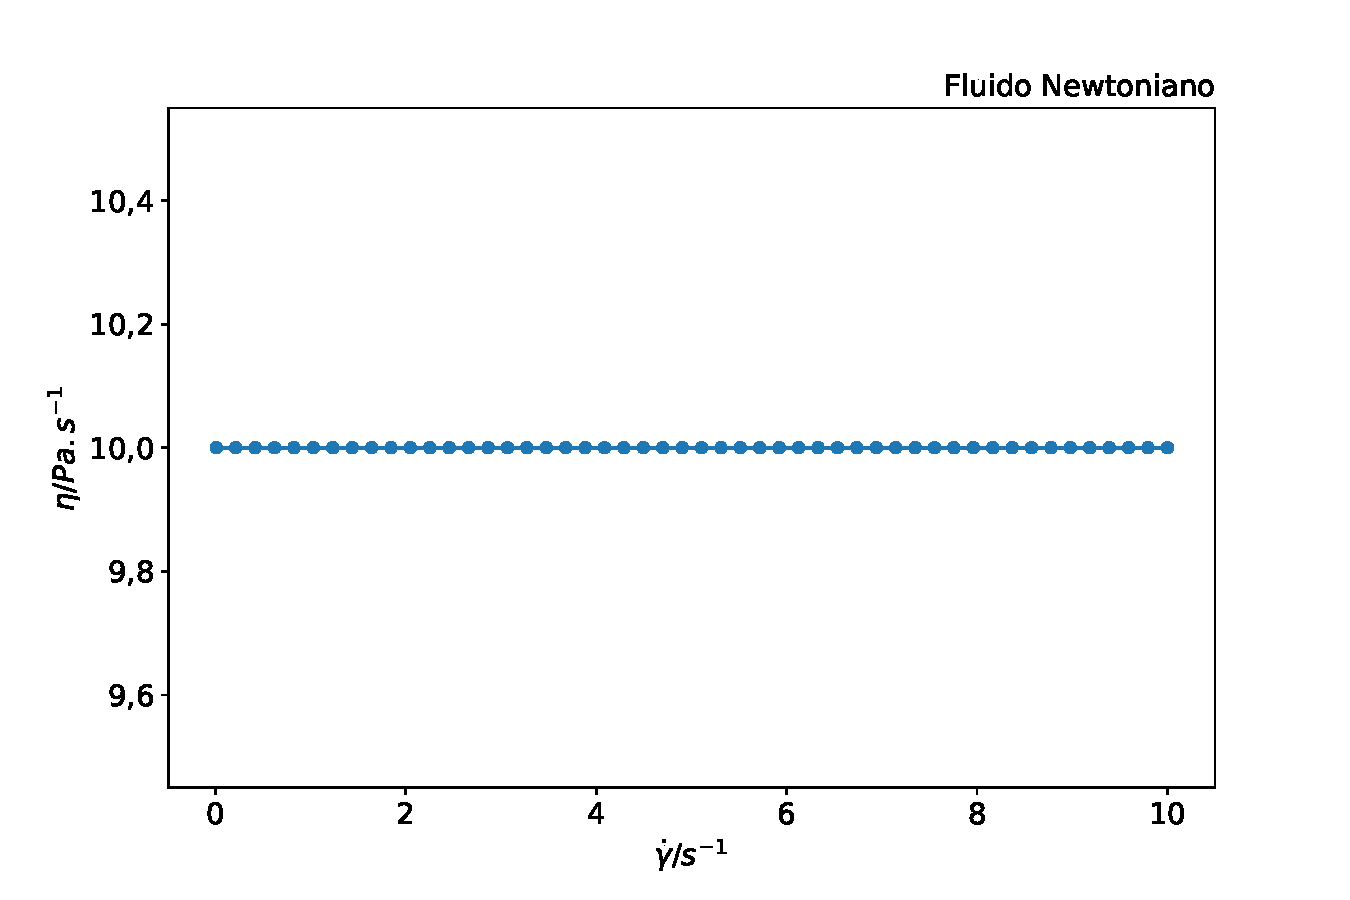
\includegraphics[width=\textwidth]{./imagens/reologia/newtoniano_exemplo_etaGP}
					\caption{\(\eta \times \dot{\gamma}\)}
					\label{fig:reol_newt_etaGP}
				\end{subfigure}
				\caption{Exemplos de curvas de fluxo. (\ref{fig:reol_newt_tauGP}) Método para obtenção da viscosidade. (\ref{fig:reol_newt_etaGP}) Dependência da viscosidade com a taxa de cisalhamento, mostrando que o valor é constante.}
				\label{fig:reol_newt_exemplos}
			\end{figure}
				
			\subsection{Sólidos Hookeanos}
			
			Sólidos hookeanos possuem uma constante elástica \(G\) que relaciona a tensão \(\tau\) aplicada e a deformação \(\gamma\) (Eq. \ref{eqn:Hooke}).
			
			\begin{equation}
				\tau = G\gamma
				\label{eqn:Hooke}
			\end{equation}
			
			A deformação de um sólido Hookeano pode ser tanto compressiva quando extensiva, dependendo do sinal de \(\gamma\), e consequentemente a tensão retornada possui a direção oposta da tensão aplicada inicialmente. 
			
			O modelo físico associado ao sólido Hookeano é a mola. É possível que uma mola, quando estendida demasiadamente, não retorne à sua extensão original. Isso ocorre porque a Eq. \ref{eqn:Hooke} se aplica somente a uma região dos possíveis valores de \(\gamma\). A fig X mostra o comportamento Hookeano de amostras.
			
			% todo: colocar uma figura do Goodwin e Hughes de viscosidade, para mostrar o comportamento não Hookeano.
			
			\subsection{Fluidos não-Newtonianos}
			
			Fluidos que não obedecem a lei de Newton (Eq. \ref{eqn:Newton}), portanto possuem valores de viscosidade dependentes da taxa de cisalhamento, são chamados de fluidos não-Newtonianos. Dentro dessa classificação, há vários tipos de fluido, dependendo de como \(\eta\) varia com (\(\dot{\gamma}\)). Alguns dos tipos possíveis são:
			
			\begin{itemize}[noitemsep]
				\item Plásticos: Viscosidade inicial é muito alta ou, teoricamente, infinita, até a tensão atingir um valor específico, chamado de tensão limite ou \emph{yield-stress}, quando o material começa a fluir. Exemplo: Manteiga, géis. % todo: achar se o termo é tensão limite mesmo
				\item Pseudoplásticos ou \emph{shear-thinning}: Viscosidade alta, mas finita, em baixas taxas de cisalhamento, e decai com o aumento da taxa de cisalhamento, atingindo um valor mínimo. Exemplo: soluções de micelas gigantes.
				\item Dilatantes: Viscosidade baixa a baixas taxas de cisalhamento, e aumenta com o aumento da taxa. Exemplo: Dispersões de amido em água.
			\end{itemize}
			
			% Todo: colocar a figura dos vários tipos de comportamento aqui.
			
			% todo: pensar melhor sobre isso de contribuições elásticas e viscosas. O que eu escrevi aqui é o oposto do que aparece no diagrama de frequência, com a viscosidade complexa. Qual é a relação?
			
			Sob taxas de cisalhamento baixas, micelas gigantes em solução estão emaranhadas. Isso dificulta a movimentação do solvente e da solução como um todo, resultado em uma viscosidade aparente alta. Nesse regime, o comportamento elástico predomina. Quanto maior for o entrelaçamento das micelas, maior é a contribuição do comportamento elástico, e maior é a viscosidade aparente. À medida que a taxa é aumentada, as micelas gigantes começam a se alinhar ao fluxo, de modo a diminuir o gradiente de velocidade que cada cadeia sente. Isso facilita o fluxo e diminui a estruturação que resulta no comportamento elástico, o que acaba diminuindo a viscosidade aparente.
			
			Após um valor específico de taxa de cisalhamento, a viscosidade atinja um mínimo pois não há mais como aumentar o alinhamento das micelas. Nessa situação, a viscosidade aparente é predominantemente devido ao solvente, e a contribuição Newtoniana é predominante. A figura \ref{fig:reol_pseudoplastico_exemplos} mostra a curva de fluxo de um material pseudoplástico, tanto .\footnote{Construção: vide apêndice \ref{sec:apn_tratamento_CF}. Parâmetros: Modelo de Carreau, \(\eta_0=10\), \(\eta_{\infty}=1\), \(\dot{\gamma}_b=10\), \(n=10\).} É possível que as cadeias comecem a se estruturar, formando \emph{shear induced structures}, mas isso não foi observado neste trabalho.
	
			\begin{figure}[H]
				\begin{subfigure}[t]{.5\textwidth}
					\includegraphics[width=\textwidth]{./imagens/reologia/pseudoplastico_tau}
					\caption{\(\tau \times \dot{\gamma}\)}
					\label{fig:reol_pseudo_tauGP}
				\end{subfigure}%
				\begin{subfigure}[t]{.5\textwidth}
					\includegraphics[width=\textwidth]{./imagens/reologia/pseudoplastico_eta}
					\caption{\(\eta \times \dot{\gamma}\)}
					\label{fig:reol_pseudo_etaGP}
				\end{subfigure}
				\caption{Exemplos de curvas de fluxo de um fluido pseudoplástico. (\ref{fig:reol_newt_tauGP}) Tensão aplicada em função da taxa de cisalhamento. (\ref{fig:reol_newt_etaGP}) Derivada de (\ref{fig:reol_newt_tauGP}) em função da taxa de cisalhamento.}
				\label{fig:reol_pseudoplastico_exemplos}
			\end{figure}
			
			No entanto, as curvas de fluxo são frequentemente plotadas na escala log-log. Nesse tipo de gráfico (Fig. \ref{fig:reol_pseudoplastico_loglog}), é possível observar a região com viscosidade constante em baixas taxas de cisalhamento, chamada de platô Newtoniano, devido à sua constância. Essa valor também é chamado de viscosidade no repouso, \(\eta_0\).
			
			\begin{figure}[H]
				\centering
				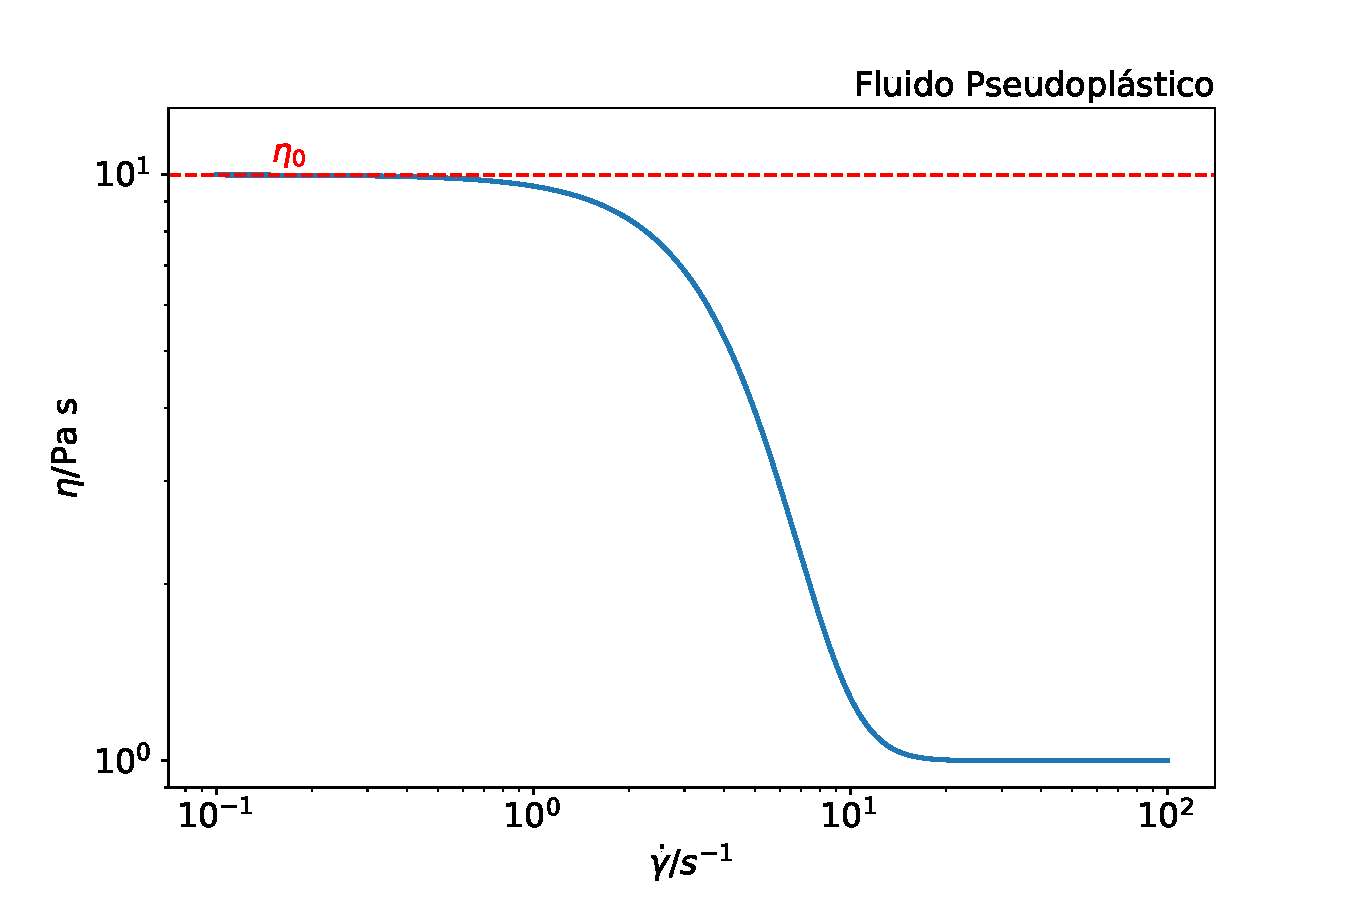
\includegraphics[width=0.7\textwidth]{./imagens/reologia/Pseudoplastico_loglog}
				\caption{Curva de fluxo de um fluído pseudoplástico na escala log-log, mostrando o valor da viscosidade no repouso, \(\eta_0\).}
				\label{fig:reol_pseudoplastico_loglog}
			\end{figure}
		
			Para obter o valor da viscosidade no repouso, é possível tanto realizar um ajuste linear da região inicial na escala log-log, ou ajustar um modelo à curva, como o modelo de Cross, Carreau e Carreau-Yasuda. Mais informações sobre a modelagem estão no apêndice \ref{sec:apn_tratamento_CF}.

		\section{Reologia oscilatória}
			\subsection{Princípios e aquisição de dados}
			
			As análises oscilatórias podem ser utilizadas para obter informações reológicas mais completas sobre um material. Variando-se a frequência de perturbação, é possível obter o espectro mecânico do material, onde se observa as contribuições elástica e viscosa em função da frequência de perturbação mecânica.
			
			Ao material, é aplicada uma deformação \(\gamma\) que varia com o tempo de acordo com a Eq. \ref{eqn:osc_gamma_t}.
			
			\begin{equation}
				\gamma(t)=\gamma_0\cos(\omega t)
				\label{eqn:osc_gamma_t}
			\end{equation}
			
			\noindent onde \(\gamma_0\) é a deformação máxima e \(\omega\) é a frequência de perturbação. As deformações aplicadas ao material devem ser tais que não ocorra desestruturação do mesmo. Por exemplo, uma deformação muito grande pode causar a quebra de ligações químicas de um polímero, o que altera irreversivelmente as suas características reológicas. Por esse motivo, é necessário modular também a tensão aplicada.
			
			Um material elástico responde à deformação imediatamente com uma força no sentido oposto ao sentido da deformação. Já materiais viscosos respondem à deformação quando há uma mudança na direção, ou seja, a resposta desses materiais é totalmente defasada em relação à aplicação da deformação. Já materiais viscoelásticos, por terem componentes de ambos os tipos, possuem uma defasagem intermediária. O grau dessa defasagem é proporcional ao grau de comportamento elástico e viscoso. Levando isso em consideração, a tensão \(\tau\)  é expressa de acordo com a Eq. \ref{eqn:osc_tau_t}.
			
			\begin{equation}
				\tau = \tau_0\cos(\omega t - \theta)
				\label{eqn:osc_tau_t}
			\end{equation}
			
			\noindent onde \(\tau_0\) é a tensão máxima (determinada no experimento oscilatório de amplitude) e \(\theta\) é o ângulo de defasagem.
			
			As expressões \ref{eqn:osc_gamma_t} e \ref{eqn:osc_tau_t} podem ser reescritas utilizando a relação de Euler, Eq. \ref{eqn:Euler}, resultando nas expressões \ref{eqn:osc_gamma_im} e \ref{eqn:osc_tau_im}, onde utilizou-se um acento circunflexo para diferenciar as expressões. Essa transformação facilita a manipulação matemática.
			
			\begin{equation}
				e^{ix} = \cos(x) + i\sin(x)
				\label{eqn:Euler}
			\end{equation}
			
			\begin{equation}
				\hat{\gamma} = \gamma_0 e^{i\omega t}
				\label{eqn:osc_gamma_im}
			\end{equation}
			
			\begin{equation}
				\hat{\tau} = \tau_0 e^{i(\omega t - \theta)}
				\label{eqn:osc_tau_im}
			\end{equation}
			
			A partir dessas relações, é possível utilizar a equação de Hooke (Eq. \ref{eqn:Hooke}) para encontrar o módulo elástico do material, na notação imaginária, \(\hat{G}\) (Eq. \ref{eqn:osc_transform_G}).
			
			\begin{equation}
				\hat{\tau} = \hat{G}\hat{\gamma} \to \hat{G} = \dfrac{\hat{\tau}}{\hat{\gamma}}    \to 
				\hat{G} = \dfrac{\tau_0}{\gamma_0} \dfrac{e^{i(\omega t - \theta)}}{e^{i\omega t}} \to
				\hat{G} = \dfrac{\tau_0}{\gamma_0} e^{-i\theta}
				\label{eqn:osc_transform_G}
			\end{equation}
			
			Utilizando-se a equação de Euler novamente, mas voltando para o domínio dos senos e cossenos, obtemos a Eq. \ref{eqn:osc_volta_senos_G}:
			
			\begin{equation}
				\hat{G} = \dfrac{\tau_0}{\gamma_0} \left( \cos(\theta) + i\sin(\theta) \right)
				\label{eqn:osc_volta_senos_G}
			\end{equation}
			
			Nessa equação, o módulo total \(\hat{G}\) foi dividido em dois termos, um em fase à deformação \(\cos(\theta)\) e outro 90° fora de fase, \(\sin(\theta)\). Esses dois termos são diretamente relacionáveis às componentes elástica e viscosa de um material. Dessa maneira, é possível separar o módulo total complexo \(\hat{G}\) em dois módulos (Eq. \ref{eqn:osc_G_complexo}), o módulo elástico, G' (Eq. \ref{eqn:osc_g1linha}), e o módulo viscoso, G'' (Eq. \ref{eqn:osc_g2linha}).
			
			\begin{equation}
				\hat{G} = G' + iG''
				\label{eqn:osc_G_complexo}
			\end{equation}
			
			\begin{equation}
				G' = \dfrac{\tau_0}{\gamma_0} \cos(\theta)
				\label{eqn:osc_g1linha}
			\end{equation}
			
			\begin{equation}
				G'' = \dfrac{\tau_0}{\gamma_0} \sin(\theta)
				\label{eqn:osc_g2linha}
			\end{equation}
			
			Portanto, para conseguir separar os valores dos módulos G' e G'', o reômetro necessita medir o módulo total e o ângulo de defasagem, sendo possível assim separar os componentes. Vale notar que a tangente do ângulo de defasagem é a relação \(G''/G'\) (Eq. \ref{eqn:osc_tan_teta})
			
			\begin{equation}
				\tan(\theta) = \dfrac{\sin(\theta)}{\cos(\theta)} = \dfrac{G''}{G'}
				\label{eqn:osc_tan_teta}
			\end{equation}
			
			A Figura \ref{fig:osc_simulacoes} mostra uma série de simulações do modelo apresentado aqui. A deformação em função do tempo foi calculada, e o ângulo de defasagem foi aumentado gradativamente de 0° para 90°. 
			% todo: descobrir e colocar os ângulos aqui
			
			\begin{figure}[H]
				\begin{subfigure}[t]{0.3\textwidth}
					\centering
					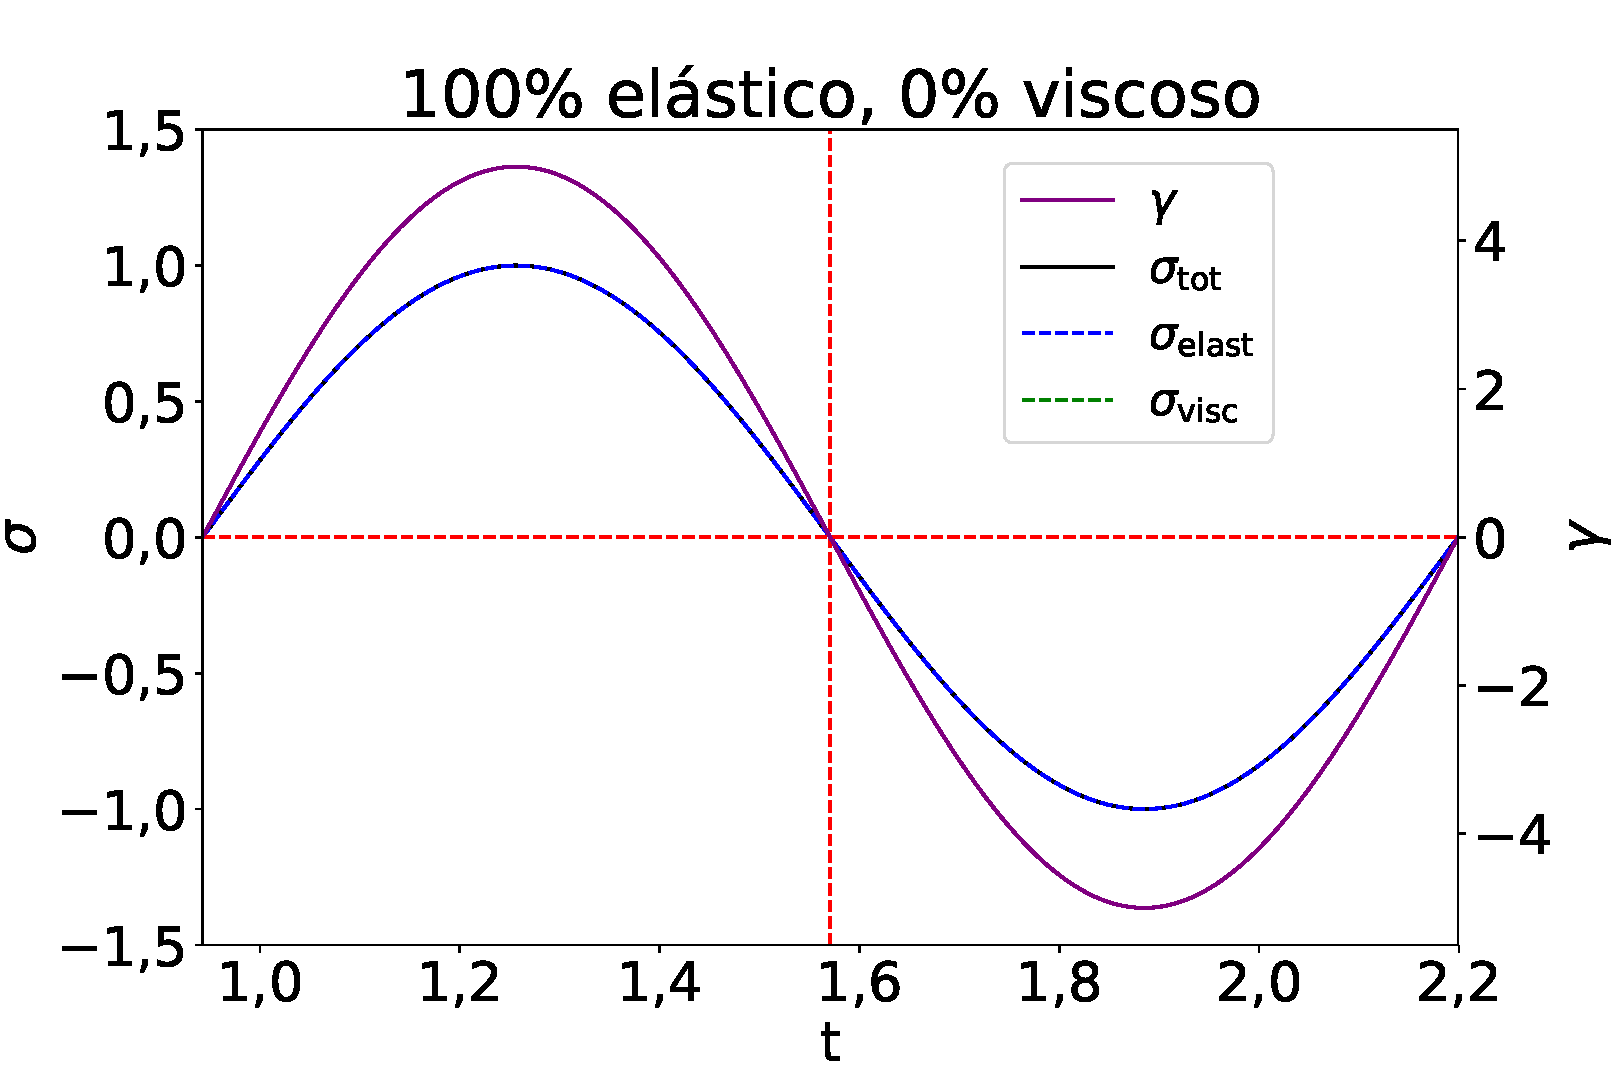
\includegraphics[width=\textwidth]{./imagens/reologia/Simulacao_visc_0}
					\caption{\(\theta=0°\)}
					\label{fig:osc_sim0}
				\end{subfigure}%
				\begin{subfigure}[t]{0.3\textwidth}
					\centering
					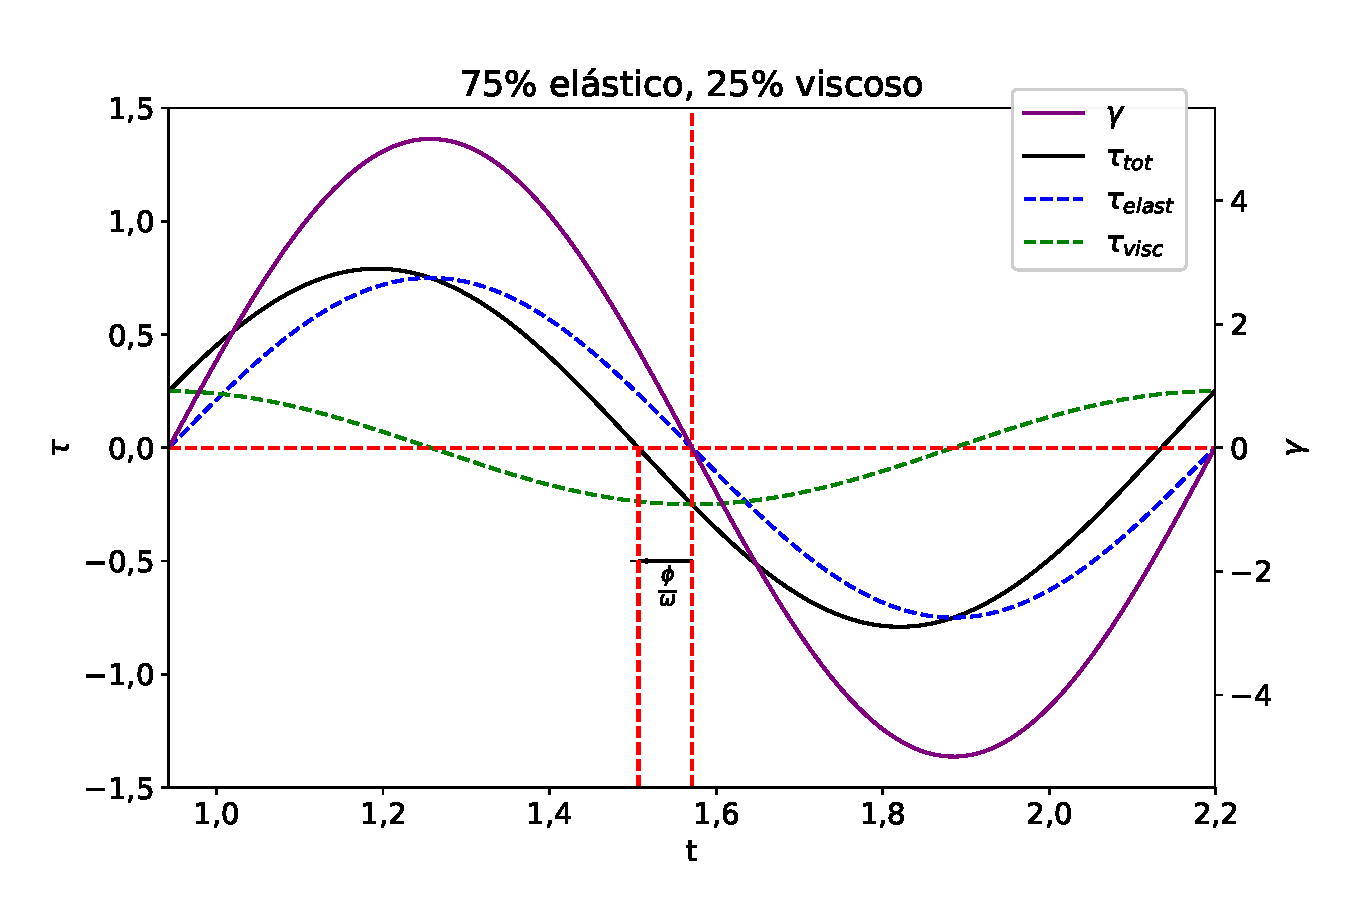
\includegraphics[width=\textwidth]{./imagens/reologia/Simulacao_visc_25}
					\caption{\(\theta=18°\)}
					\label{fig:osc_sim25}
				\end{subfigure}%
				\begin{subfigure}[t]{0.3\textwidth}
					\centering
					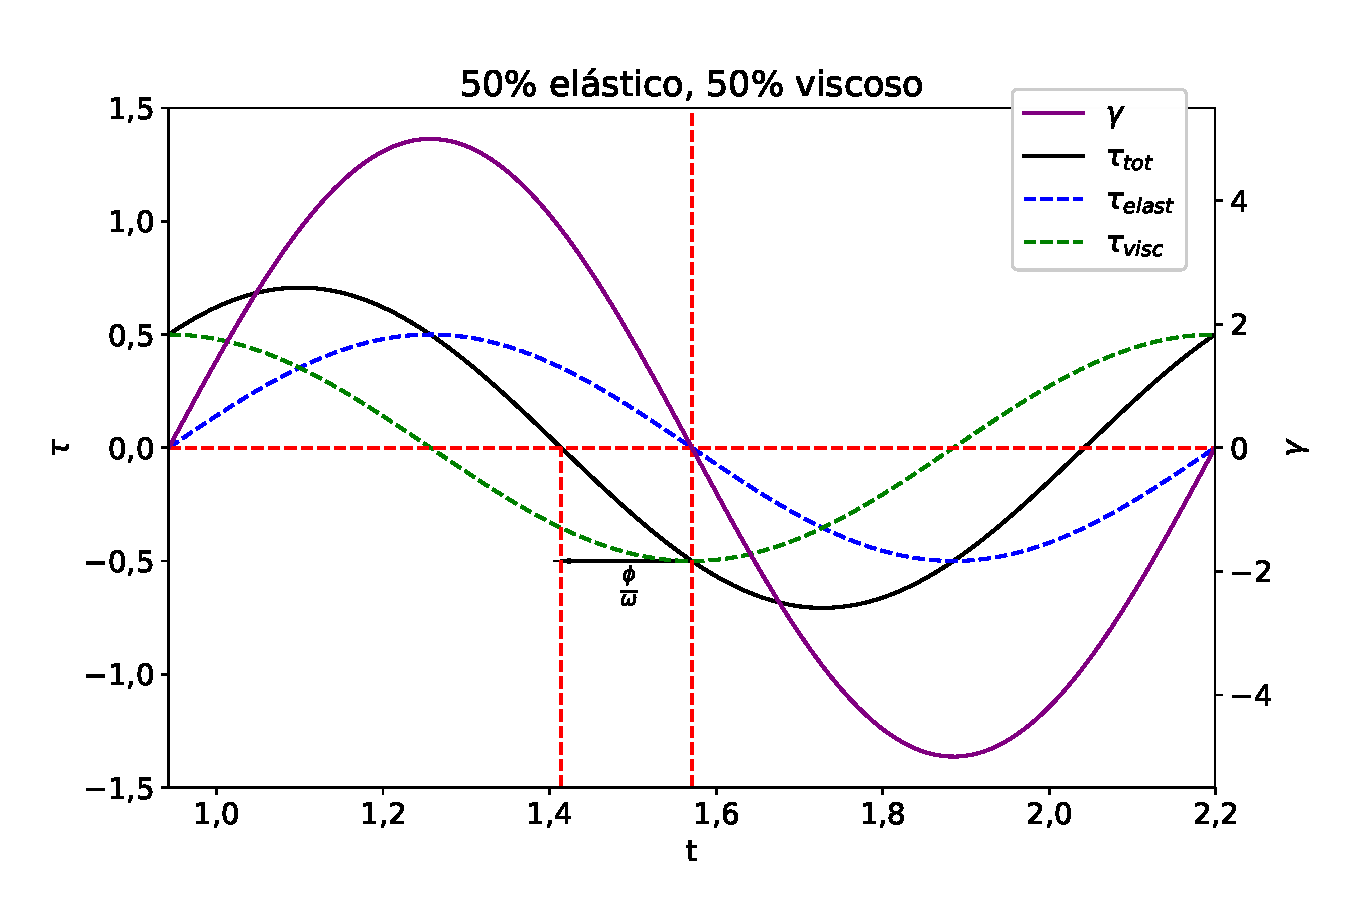
\includegraphics[width=\textwidth]{./imagens/reologia/Simulacao_visc_50}
					\caption{\(\theta=45°\)}
					\label{fig:osc_sim50}
				\end{subfigure}
			
				\begin{subfigure}[t]{0.3\textwidth}
					\centering
					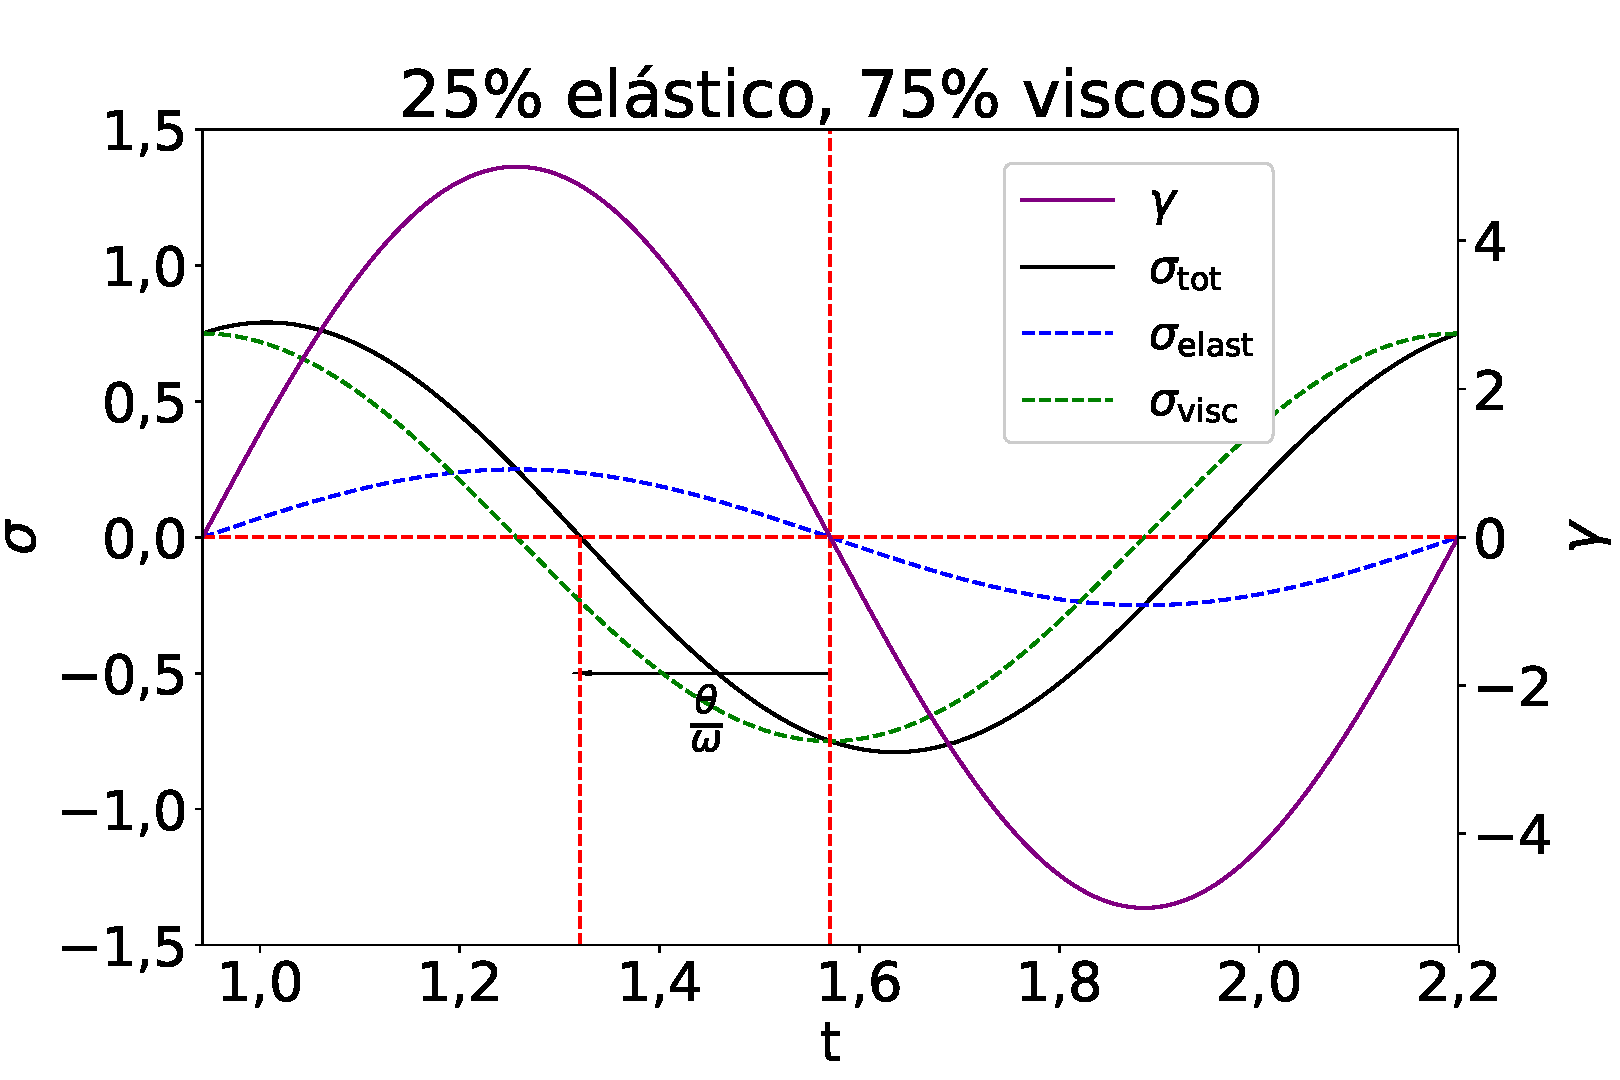
\includegraphics[width=\textwidth]{./imagens/reologia/Simulacao_visc_75}
					\caption{\(\theta=72°\)}
					\label{fig:osc_sim75}
				\end{subfigure}%
				\begin{subfigure}[t]{0.3\textwidth}
					\centering
					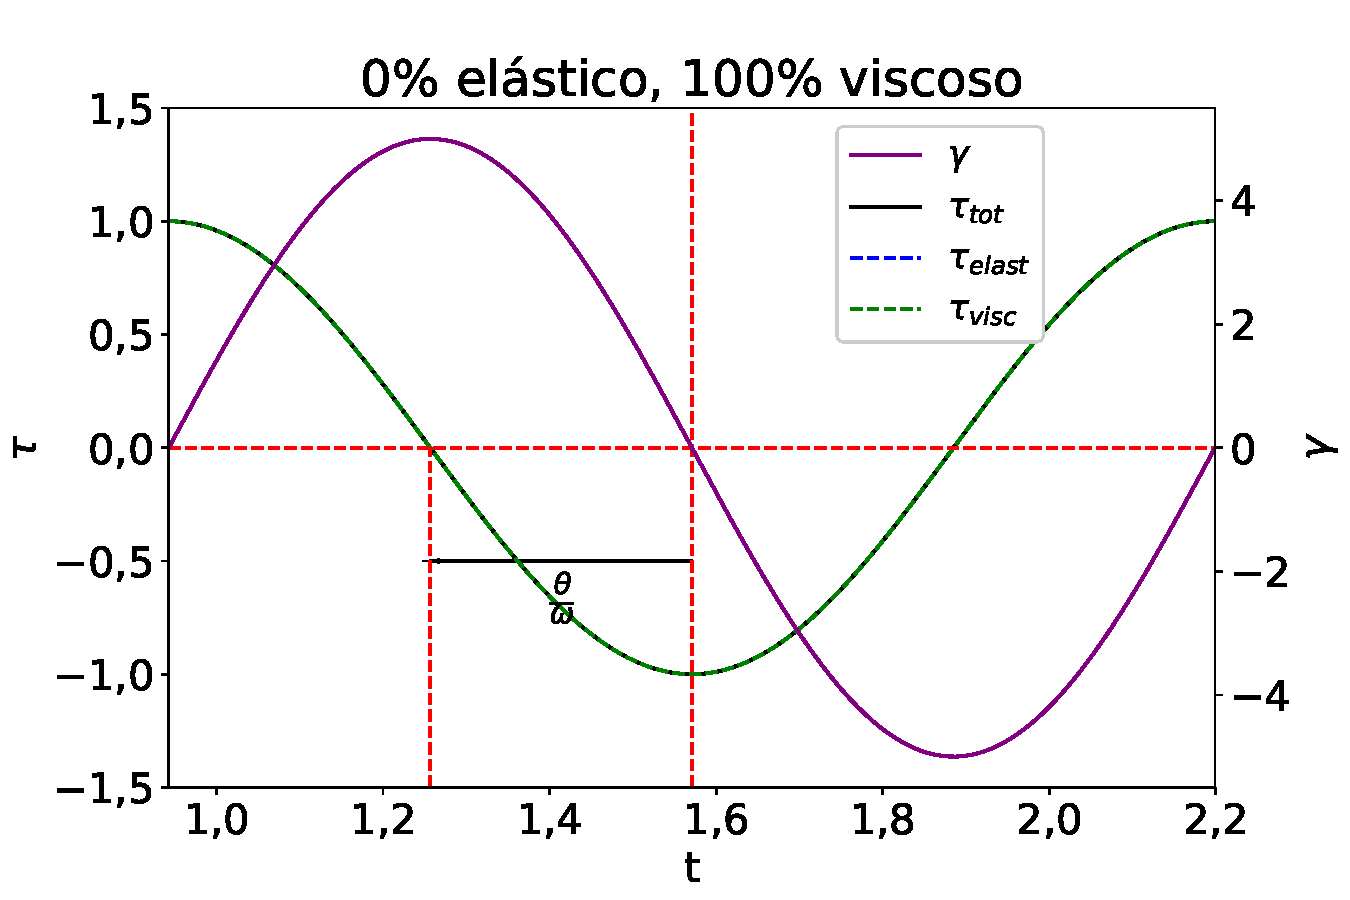
\includegraphics[width=\textwidth]{./imagens/reologia/Simulacao_visc_100}
					\caption{\(\theta=90°\)}
					\label{fig:osc_sim100}
				\end{subfigure}%
%				\begin{subfigure}[t]{0.3\textwidth}
%					\centering
%					\includegraphics[width=\textwidth]{}
%					\label{fig:}
%				\end{subfigure}
			\caption{Simulações do comportamento de um fluido sob cisalhamento cossenoidal. As imagens mostram a deformação \(\gamma\) em função do tempo, a tensão total \(\tau\) de resposta em função do tempo, decomposta em suas componentes elástica e viscosa. No título de cada gráfico está a contribuição, em porcentagem, de cada componente do material. O ângulo de defasagem está ilustrado na figura.}
			\label{fig:osc_simulacoes}
			\end{figure}  % todo: colocar o código para essa figura nos apêndices
			
			\subsection{Modelo de Maxwell}
			
			O modelo de Maxwell é construído juntando-se um elemento elástico (mola) e um elemento viscoso (dissipador), ideais, em série. A Figura \ref{fig:ilust_modelo_maxwell} ilustra essa construção.
			
			\begin{figure}[H]
				\centering
				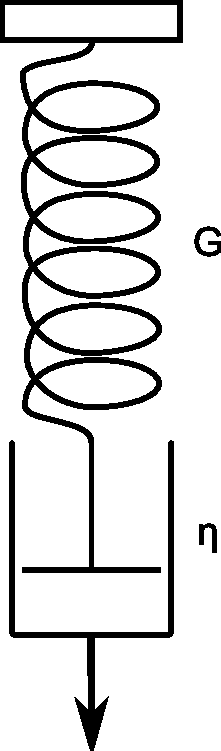
\includegraphics[width=1.5cm]{./imagens/reologia/maxwell_mola_dissipador}
				\caption{Modelo de Maxwell: Mola com constante elástica \(G\) e dissipador com constante viscosa \(\eta\) em série}
				\label{fig:ilust_modelo_maxwell}
			\end{figure}

			 É possível expressar a taxa de cisalhamento do modelo de Maxwell como a soma das taxas de cisalhamento dos elementos individuais (Eq. \ref{eqn:Maxwell_soma}). 
			 
			\begin{equation}
				\dot{\gamma}_{\textrm{total}} =  \dot{\gamma}_{\textrm{viscoso}} + \dot{\gamma}_{\textrm{elástico}} \to
				\dfrac{d\gamma}{dt} = \dfrac{1}{\eta}\tau + \dfrac{1}{G}\dfrac{d\tau}{dt}
				\label{eqn:Maxwell_soma}
			\end{equation}
			
			Para uma deformação constante, \(\frac{d\gamma}{dt}=0\), a Eq. \ref{eqn:Maxwell_soma} se torna uma equação diferencial (Eq. \ref{eqn:Maxwell_diferencial}).
			
			\begin{equation}
				\dfrac{1}{\eta}\tau + \dfrac{1}{G}\dfrac{d\tau}{dt} = 0
				\label{eqn:Maxwell_diferencial}
			\end{equation}
			
			Utilizando as condições de contorno necessárias, essa equação pode ser resolvida, resultando em (Eq. \ref{eqn:Maxwell_dif_resolvida}):
			
			\begin{equation}
				\tau(t) = \tau_0 e^{\left( -\frac{G}{\eta}t \right)}
				\label{eqn:Maxwell_dif_resolvida}
			\end{equation}
			
			O termo exponencial na Eq. \ref{eqn:Maxwell_dif_resolvida} possui unidade de tempo e é a relação entre as componentes elástica e viscosa do material. Essa relação recebe o nome de tempo de relaxação, \(\tau_{\textrm{rel}}\) (Eq. \ref{eqn:Maxwell_tempo_rel_def})
			
			\begin{equation}
				\tau(t) = \tau_0 e^{\sfrac{-t}{\tau_{\textrm{rel}}}}
				\label{eqn:Maxwell_tempo_rel_def}
			\end{equation}
		
			O tempo de relaxação é o tempo em que a tensão inicial demora para cair ao valor de \(\sfrac{1}{e}\) do valor inicial. É interessante notar que em tempos pequenos, relativos a \(\tau_{\textrm{rel}}\), o material responde com a tensão inicial total. Essa é a resposta imediata da mola. Porém, com o tempo, à medida que \(t\to\tau_{\textrm{rel}}\), a tensão começa a decair exponencialmente e depois, em \(t \gg \tau_{\textrm{rel}}\), tende a zero. Nessa situação, o dissipador difundiu toda a energia inicial aplicada.
			
			A expressão \ref{eqn:Maxwell_soma} pode ser rearranjada utilizando o tempo de relaxação (\ref{eqn:Maxwell_tempo_rel_def}).
			
			\begin{equation}
				\dfrac{d\gamma}{dt} = \dfrac{1}{\eta}\tau + \dfrac{1}{G}\dfrac{d\tau}{dt} \to 
				\tau = -\dfrac{\eta}{G} \dfrac{d\tau}{dt} + \eta\dfrac{d\gamma}{dt} =
				-\tau_{\textrm{rel}} \dfrac{d\tau}{dt} + \eta\dfrac{d\gamma}{dt}
				\label{eqn:Maxwell_inicio_g1g2}
			\end{equation}
			
			É possível substituir as expressões de tensão e \ref{eqn:osc_gamma_im} e \ref{eqn:osc_tau_im} na expressão \ref{eqn:Maxwell_inicio_g1g2} para obter uma expressão em função do tempo, da frequência e do ângulo de fase. Já realizando as derivações, obtemos:
			
			\begin{equation}
				\tau_0 e^{i \left( \omega t - \theta \right)} = - \tau_{\textrm{rel}} \tau_0 i\omega e^{i \left( \omega t - \theta \right)}     +       \eta i\omega\gamma_0e^{i\omega t}
				\label{eqn:Maxwell_substituicao}
			\end{equation}
			
			Em comum a todos os termos é a constante \(e^{i\omega t}\). Dividindo ambos os lados por essa constante, agrupando os termos com \(e^{-i\theta}\) e substituindo a viscosidade por \(G\tau_{\textrm{rel}}\), temos:
			
			\begin{equation}
				\tau_0e^{-i\theta} \left(   1 + i\omega\tau_{\textrm{rel}}  \right) = i\omega G\tau_{\textrm{rel}}\gamma_0 \to
				\tau_0e^{-i\theta} = \dfrac{i\omega G\tau_{\textrm{rel}}\gamma_0}{\left(   1 + i\omega\tau_{\textrm{rel}}  \right)}
				\label{eqn:Maxwell_intermediario}
			\end{equation}
			
			O termo à esquerda da Eq. \ref{eqn:Maxwell_intermediario} é similar à definição do módulo elástico complexo, Eq. \ref{eqn:osc_transform_G}, sendo necessário somente dividir ambos os lados por \(\gamma_0\). Realizando a substituição, temos:
			
			\begin{equation}
				\hat{G} = \dfrac{\tau_0e^{-i\theta}}{\gamma_0} = \dfrac{i\omega G\tau_{\textrm{rel}}}{\left(   1 + i\omega\tau_{\textrm{rel}}  \right)}
				\label{eqn:Maxwell_complexo_antes_sep}
			\end{equation}
			
			Seguindo o princípio de que o módulo complexo \(\hat{G}\) pode ser dividido em uma parte imaginária e uma parte real, podemos realizar o mesmo com a Eq. \ref{eqn:Maxwell_complexo_antes_sep} multiplicando-se a fração por \(\frac{\left(   1 - i\omega\tau_{\textrm{rel}}  \right)}{\left(   1 - i\omega\tau_{\textrm{rel}}  \right)}\).
			
			\begin{equation}
				\hat{G} = \dfrac{  i\omega G\tau_{\textrm{rel}} - i^2 \omega^2 G \tau_{\textrm{rel}}^2        }{  1 - i^2\omega^2 \tau_{\textrm{rel}}^2          }
				\label{eqn:Maxwell_complexo_antes_sep2}
			\end{equation}
			
			Separando as partes imaginárias das partes reais e substituindo \(i^2 = -1\):
			
			\begin{equation}
				\hat{G} = \dfrac{   \omega^2 G \tau_{\textrm{rel}}^2       }{  1 + \omega^2 \tau_{\textrm{rel}}^2      } + i \dfrac{   \omega G \tau_{\textrm{rel}}        }{ 1 + \omega^2 \tau_{\textrm{rel}}^2 }
				\label{eqn:Maxwell_substituido}
			\end{equation}
			
			Seguindo a expressão \ref{eqn:osc_G_complexo}, \(\hat{G} = G' + iG''\), podemos definir o módulo elástico de acordo com o modelo de Maxwell como:
			
			\begin{equation}
				G' = \dfrac{ G \omega^2 \tau_{\textrm{rel}}^2   }{  1 + \omega^2 \tau_{\textrm{rel}}^2      }
				\label{eqn:Maxwell_G1_def}
			\end{equation}
			
			E o módulo viscoso, G'', como:
			
			\begin{equation}
				G'' = \dfrac{  G \omega  \tau_{\textrm{rel}}        }{ 1 + \omega^2 \tau_{\textrm{rel}}^2 }
				\label{eqn:Maxwell_G2_def}
			\end{equation}
			
			É interessante notar que a relação \(\sfrac{G''}{G'}\), que equivale a \(\tan(\theta)\) (\ref{eqn:osc_tan_teta}), também se relaciona com o tempo de relaxação:
			
			\begin{equation}
				\tan(\theta) = \dfrac{G''}{G'} = \dfrac{1}{\omega\tau_{\textrm{rel}}}
				\label{eqn:Maxwell_cruzamento}
			\end{equation}
			
			Com isso, é possível determinar o tempo de relaxação de um fluido Maxwelliano através da frequência do ponto de cruzamento de G' e G''. Lembrando que \(\omega\) é a frequência de perturbação, e o inverso da frequência é o tempo de observação, podemos relacionar essa relação com o número de Deborah, Eq. \ref{eqn:Deborah}.
			
			\begin{equation}
				\dfrac{1}{\omega\tau_{\textrm{rel}}} = \dfrac{ t_{\textrm{observação}  }}{ \tau_{\textrm{rel}}  } = \dfrac{1}{D_e}
				\label{eqn:Maxwell_cruzamento_Deborah}
			\end{equation}

			A reologia oscilatória geralmente é expressa em termos de G' e G'' em função da frequência, na escala logarítmica. A Fig. \ref{fig:modelo_maxwell} mostra duas curvas simuladas para um material com tempo de relaxação de 10 s.$rad^{-1}$ e um módulo \(G\) de 10 Pa. Nessa figura estão mostrado como se obtêm visualmente os parâmetros \(G\) e \(\tau_{\textrm{rel}}\).
			
			\begin{figure}[H]
				\centering
				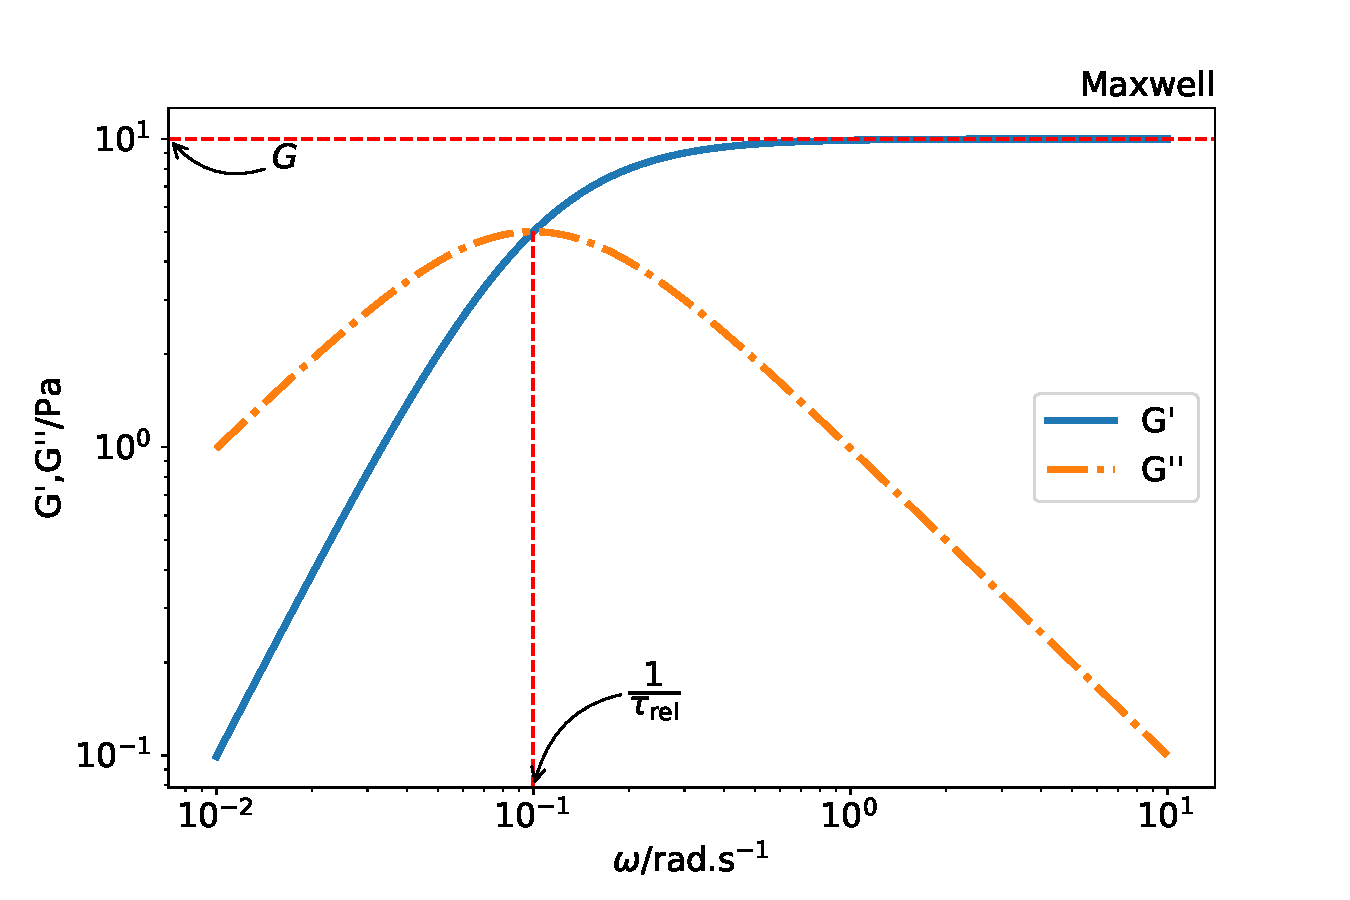
\includegraphics[width=0.7\textwidth]{./imagens/reologia/modelo_maxwell}
				\caption{Espectro mecânico de acordo com o modelo de Maxwell}
				\label{fig:modelo_maxwell}
			\end{figure}
						
			Micelas gigantes, em vários regimes, obedecem muito bem o modelo de Maxwell. É possível interpretar esse comportamento da seguinte maneira. Em baixas frequências de perturbação (longos tempos), as micelas possuem tempo suficiente para deslizar umas pelas outras, então a maior parte da energia fornecida é perdida, logo o módulo viscoso, ou de perda, possui valores altos. Em frequências altas, a rede micelar e os entrelaçamentos conseguem armazenar a energia, não possuindo tempo suficiente para deslizar, então o módulo elástico, ou de armazenamento, é alto. Na região intermediária, ambos os mecanismos estão presentes, parte da energia é perdida e parte é armazenada, sendo que no ponto de cruzamento, exatamente metade da energia é preservada e metade é perdida.
			
			Para a obtenção de valores mais confiáveis para os parâmetros, é necessário realizar um ajuste dessas curvas. Porém, existem duas curvas que são descritas pelos mesmos parâmetros. Ao invés de se fazer dois ajustes e encontrar quatro parâmetros, é ideal realizar um ajuste das duas curvas simultaneamente. Isso pode ser feito minimizando-se um vetor com os resíduos das duas curvas concatenados. Isso pode ser feito utilizando-se, por exemplo, o Excel, com a ferramenta \emph{Solver} para minimizar o resíduo.
			
			\subsection{Modelos mais complexos}
			
			Experimentalmente, existem divergências entre o modelo de Maxwell e os espectros mecânicos dos materiais. Geralmente, essas divergências aparecem devido ao aparecimento de outros  mecanismos de relaxação em frequências mais altas. Para isso, existem alguns modelos que visam corrigir o modelo de Maxwell, afetando principalmente essa região.
			
			Uma possível correção é utilizar dois elementos de Maxwell em série, produzindo um modelo que tem dois tempos de relaxação e dois módulos (Eqs. \ref{eqn:modelo_doismodos_g1}, \ref{eqn:modelo_doismodos_g2}).
			
			\begin{equation}
				G' = \dfrac{ G_1 \omega^2 \tau_{\textrm{rel,1}}^2   }{  1 + \omega^2 \tau_{\textrm{rel,1}}^2      } + \dfrac{ G_2 \omega^2 \tau_{\textrm{rel,2}}^2   }{  1 + \omega^2 \tau_{\textrm{rel,2}}^2      }
			\label{eqn:modelo_doismodos_g1}
			\end{equation}
		
			\begin{equation}
				G'' = \dfrac{  G_1 \omega  \tau_{\textrm{rel,1}}        }{ 1 + \omega^2 \tau_{\textrm{rel,1}}^2 } + \dfrac{  G_2 \omega  \tau_{\textrm{rel,2}}        }{ 1 + \omega^2 \tau_{\textrm{rel,2}}^2 }
			\label{eqn:modelo_doismodos_g2}
			\end{equation}
			
			% todo: a viscosidade do Oldroyd é para isso mesmo?
			
			O modelo de Oldroyd é praticamente idêntico ao modelo de Maxwell, e introduz somente um termo relativo à viscosidade do solvente para altas frequências de G'' (Eq. \ref{eqn:modelo_oldroyd_g2}). G' é inalterado.
			
			\begin{equation}
				G'' =\dfrac{  G \omega  \tau_{\textrm{rel}}        }{ 1 + \omega^2 \tau_{\textrm{rel}}^2 } + \eta_{\infty} * \omega
				\label{eqn:modelo_oldroyd_g2}
			\end{equation}
			
			O modelo mais diferente do modelo de Maxwell é o modelo de Jeffreys, que possui as seguintes formas:
			
			\begin{equation}
				G' = \dfrac{G \omega^{2} \tau_{\textrm{rel,1}} \left(\tau_{\textrm{rel,1}} - \tau_{\textrm{rel,2}}\right)}{1 + \omega^{2} \tau_{\textrm{rel,1}}^{2}}
				\label{eqn:modelo_jeffreys_g1}
			\end{equation}
			
			\begin{equation}
				G'' = \dfrac{G \omega \tau_{\textrm{rel,1}} \left(\omega^{2} \tau_{\textrm{rel,1}} \tau_{\textrm{rel,2}} + 1\right)}{1 + \omega^{2} \tau_{\textrm{rel,1}}^{2}}
				\label{eqn:modelo_jeffreys_g2}
			\end{equation}
			
			% todo: verificar na literatura essas equações.
			
			A Figura \ref{fig:comparativo_modelos} compara os três modelos mais complexos apresentados com o modelo de Maxwell. 
			
			\begin{figure}[H]
				\begin{subfigure}[t]{.5\textwidth}
					\centering
					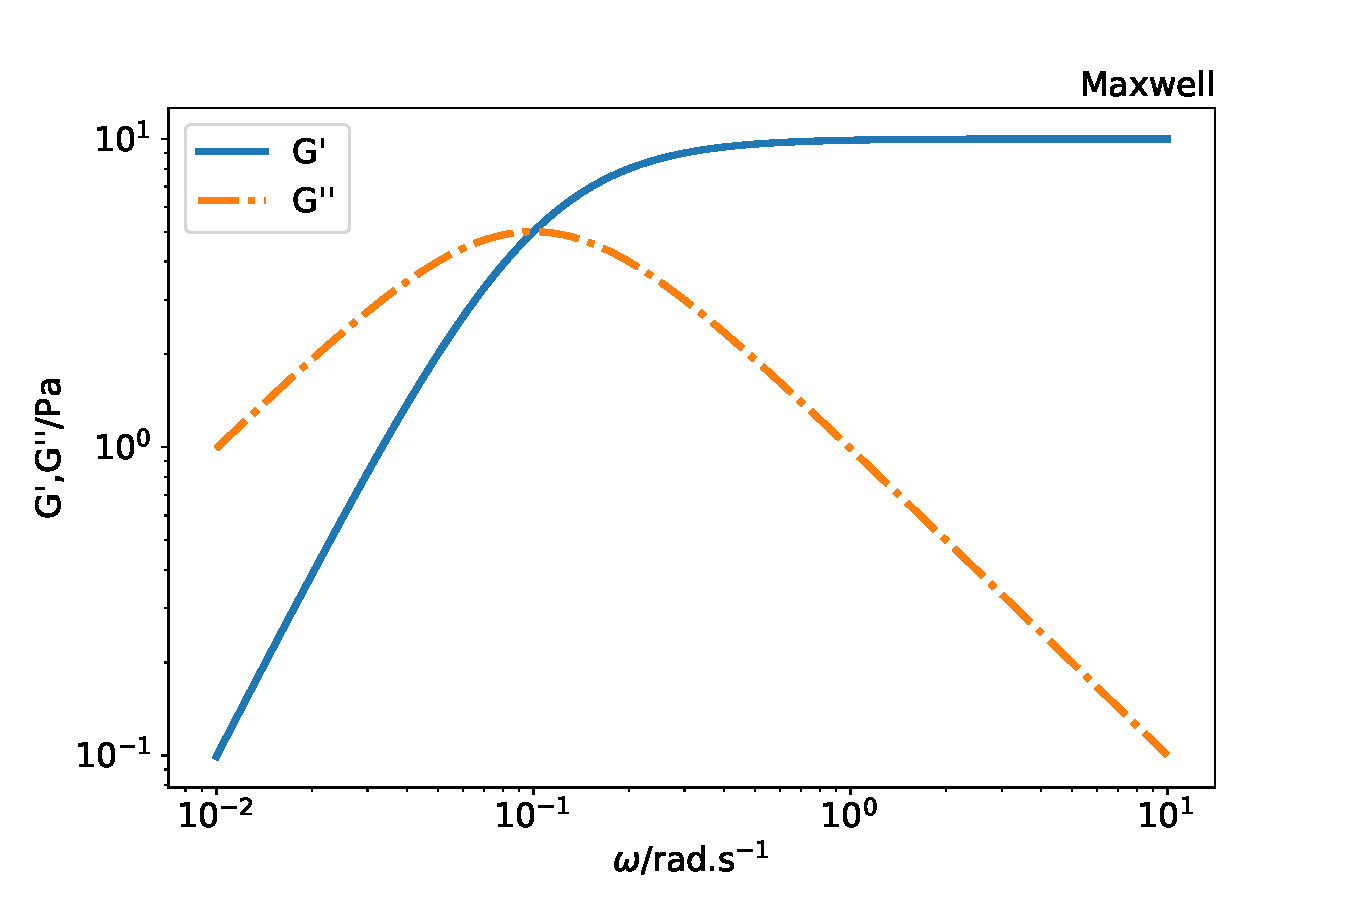
\includegraphics[width=\textwidth]{./imagens/reologia/modelos_comparativo_max}
					\caption{Maxwell. \(G=10, \tau_{\textrm{rel}}=10\)}
					\label{fig:comparativo_modelo_maxwell}
				\end{subfigure}%
				\begin{subfigure}[t]{.5\textwidth}
					\centering
					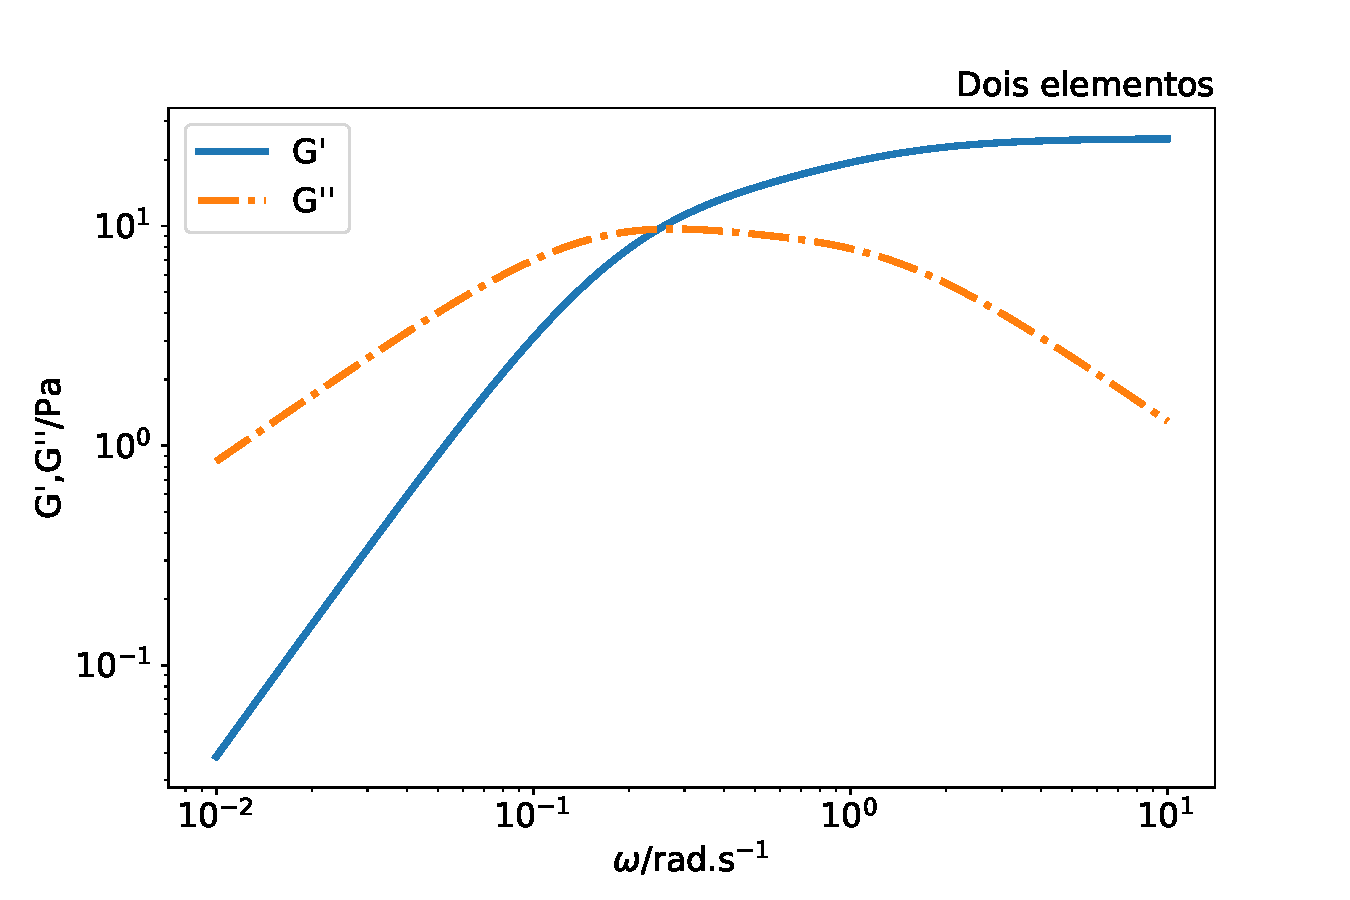
\includegraphics[width=\textwidth]{./imagens/reologia/modelos_comparativo_doismodos}
					\caption{Dois Módulos. \(G_1=10, G=15, \tau_{\textrm{rel,1}}=1,  \tau_{\textrm{rel,2}}=5\)}
					\label{fig:comparativo_modelo_doismodos}
				\end{subfigure}
			
				\begin{subfigure}[t]{.5\textwidth}
					\centering
					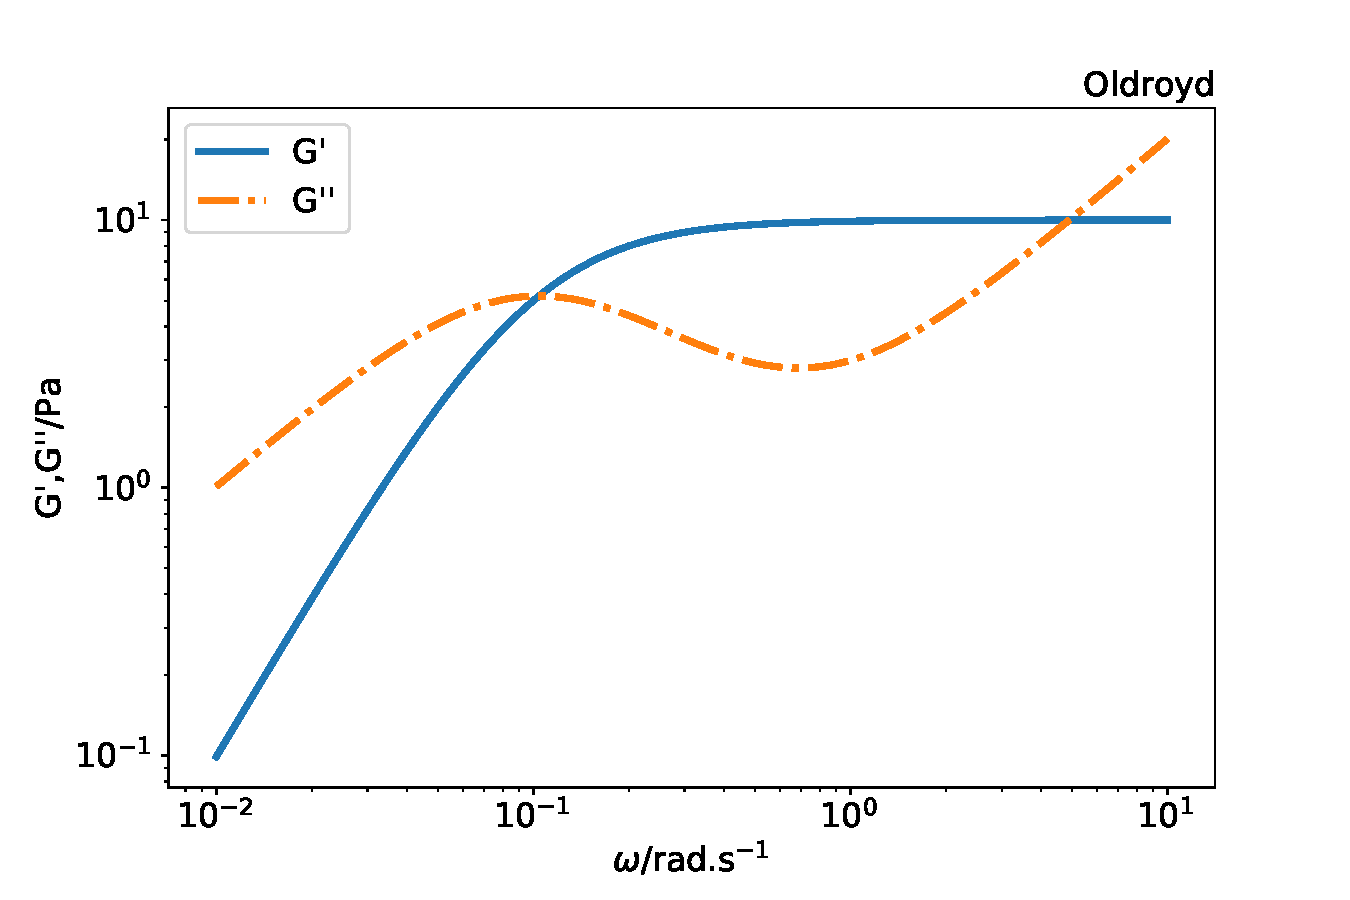
\includegraphics[width=\textwidth]{./imagens/reologia/modelos_comparativo_oldroyd}
					\caption{Oldroyd. \(G=10, \tau_{\textrm{rel}}=10, \eta_{\infty}=2\)}
					\label{fig:comparativo_modelo_oldroyd}
				\end{subfigure}%	
				\begin{subfigure}[t]{.5\textwidth}
					\centering
					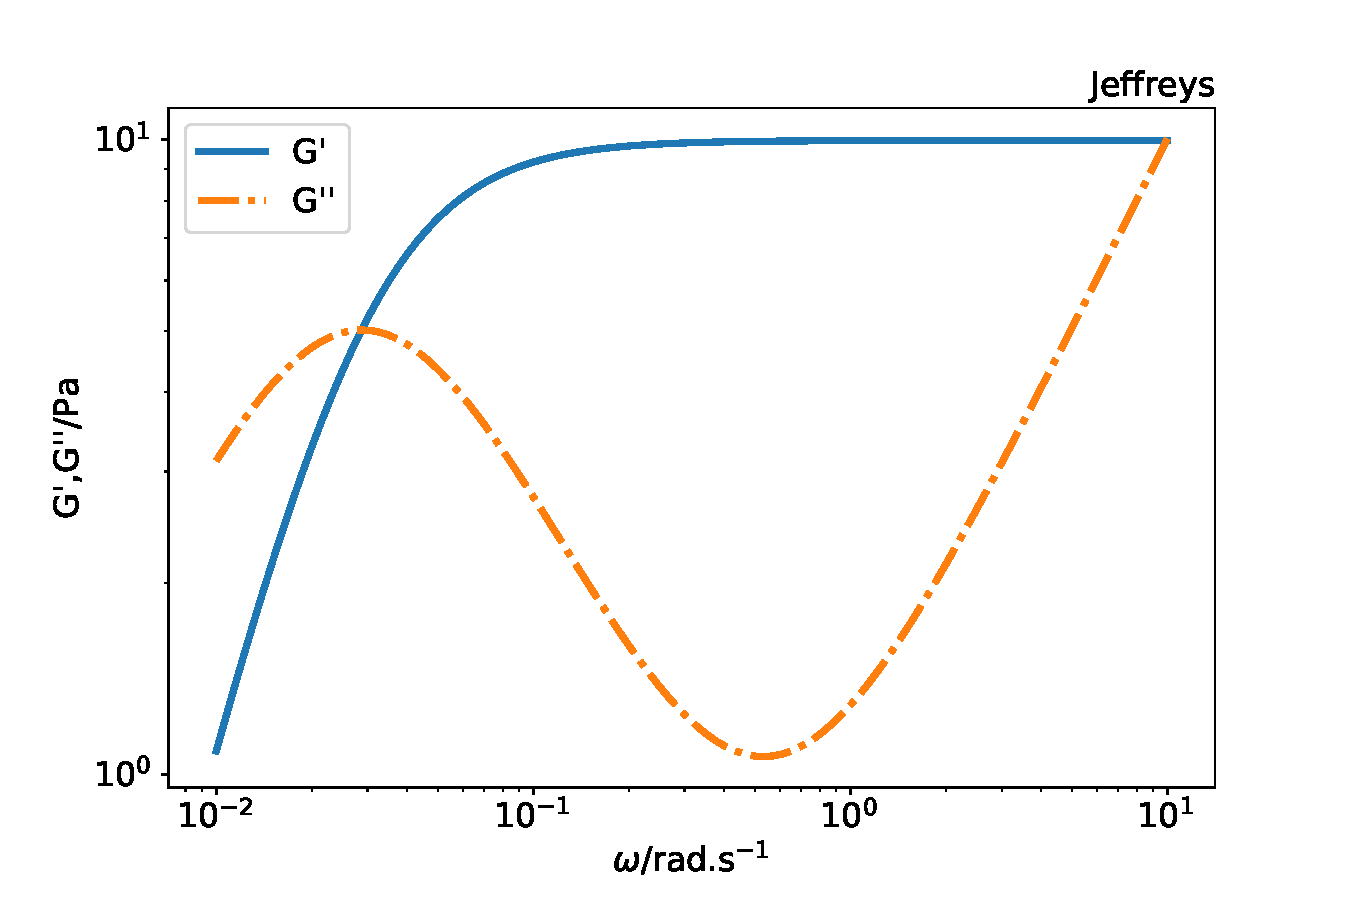
\includegraphics[width=\textwidth]{./imagens/reologia/modelos_comparativo_jeffreys}
					\caption{Jeffreys. \(G=10, \tau_{\textrm{rel,1}}=35, \tau_{\textrm{rel,2}}=0.1 \)}
					\label{fig:comparativo_modelo_jeffreys}
				\end{subfigure}
			
				\caption{Comparação dos modelos de Maxwell, Dois-Módulos, Oldroyd e Jeffreys. Nas legendas estão os parâmetros para a criação dos modelos. Os módulos estão na unidade de Pa, os tempos de relaxação, em \(s.rad^{-1}\) e \(\eta_{\infty}\) em Pa.s}
				\label{fig:comparativo_modelos}
			\end{figure}
			
			% todo: pensar se eu devo descrever os detalhes de micelas gigantes aqui, ou na seção de micelas mesmo.
			% todo: colocar o modelo de García-Saraji
	\chapter{Calorimetria de titulação isotérmica}
	
		\section{Fundamentos}
		
		% todo: encontrar um termo melhor para ``caixa adiabática''
		
		A calorimetria de titulação isotérmica (ITC) é uma técnica baseada na liberação ou absorção de calor durante um processo de titulação. Há duas celas dentro de uma caixa adiabática, uma de referência, que contém somente água, e outra de amostra, onde ocorre a titulação em si. A cela de referência recebe uma quantidade fixa de calor através de uma resistência, e a cela de amostra recebe uma quantidade variável de calor. A figura \ref{fig:ITC_esquema} ilustra a construção de um calorímetro.
		
		\begin{figure}[h]
			\centering
			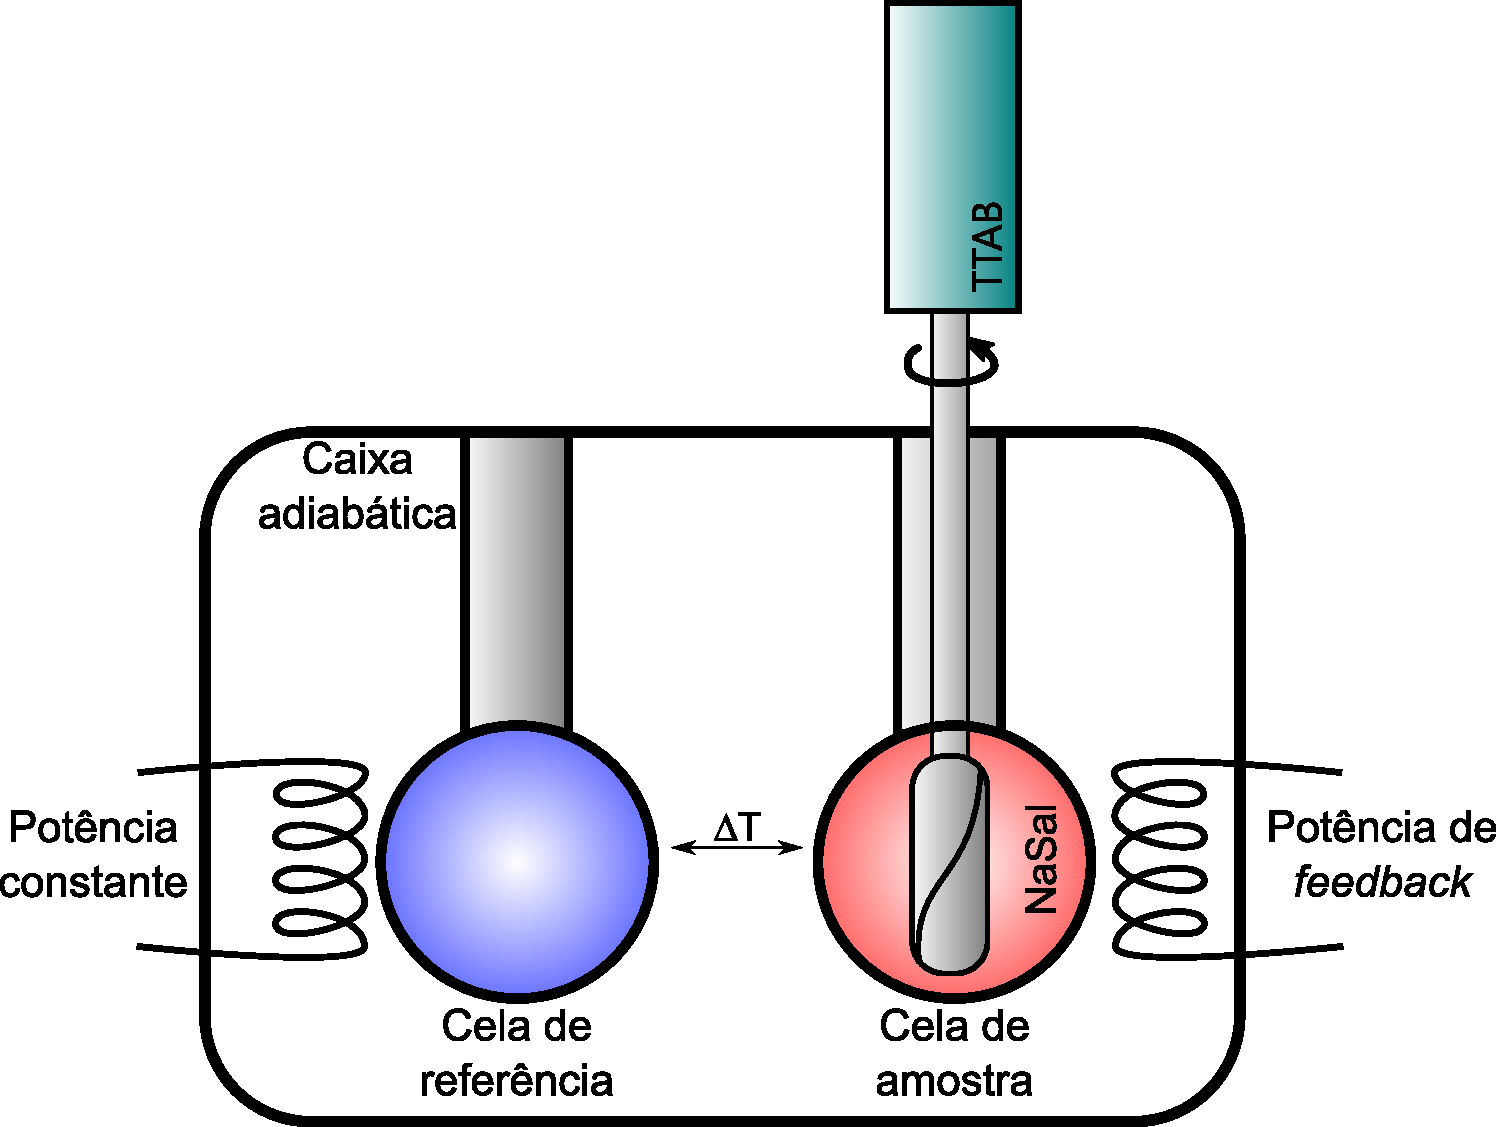
\includegraphics[width=0.5\textwidth]{./imagens/itc/esquema_itc_equipamento}
			\caption{Esquema da construção de um calorímetro de titulação isotérmica}
			\label{fig:ITC_esquema}
		\end{figure}
		
		Durante uma titulação, caso ocorra liberação de calor na cela de amostra, menos energia, em relação ao valor basal, precisa ser fornecida para manter a temperatura igual entre as celas. Caso o sistema absorva energia, mais potência precisa ser fornecida à cela. Esse comportamento se expressa em picos positivos e negativos. A integração de cada pico no tempo fornece valores de energia que, quando divididos pelo número de mols injetados, obtemos valores de $\Delta H^0/kJ.mol^{-1}$ [X, Y]. A Figura \ref{fig:ITC_esquema} mostra esse processo.
		
		%\cite{Loh2016, Grolier2012}
		% Processo de aquisição de um entalpograma. Uma solução de TTAB é titulada em NaSal (esquerda). A potência de \emph{feedback} responde ao $\Delta T$ formado entre a cela de referência e amostra (centro). A potência em função do tempo é integrada e dividida pela quantidade de TTAB adicionado por injeção, resultando no entalpograma (direita).
		%%%%%%%%%%
		Para micelas gigantes, fixa-se uma concentração de aditivo e depois surfactante é titulado. O padrão da curva de $\Delta H \times C_{\textsf{surf}}$ é bastante característico. No início há muito NaSal e pouco TTAB, e ocorre a formação de micelas esféricas com NaSal. À medida que mais NaSal é incorporado, são formadas micelas mistas cilíndricas curtas . Numa determinada concentração, ocorre uma queda bastante brusca no valor de $\Delta H$, devido à fusão de várias micelas cilíndricas, formando micelas gigantes. A diferença de entalpia entre os estados final e inicial dessa queda brusca caracteriza $\Delta H_{\mathsf{WLM}}$. A concentração no ponto mínimo caracteriza $c_{\mathsf{WLM}}$\cite{Ito2016}.
		
		Com a técnica de ITC, pode-se observar o quão favorável é a formação de micelas gigantes em determinadas condições. Quanto menor for $c_{\mathsf{WLM}}$, mais favorável é a formação das micelas. A $c_{\mathsf{WLM}}$ é referente ao grau de incorporação de aditivo na etapa de formação de micelas\cite{Ito2016}.
		
		
			\subsection{Aquisição de dados}
		\section{Calorimetria de micelas esféricas}
		\section{Calorimetria de micelas gigantes}
		\section{Termodinâmica de micelização}
	\chapter{SAXS}
		\section{Fundamentos}
		\section{Modelagem}
			\subsection{Esferas}
			\subsection{Micelas esféricas}
			\subsection{Micelas gigantes}
			\subsection{Visualização dos parâmetros}
			\subsection{Indexação de picos}
	\chapter{Fluorescência}
		\section{Fundamentos}
			\subsection{Diagramas}
			\subsection{Rendimento quântico}
			\subsubsection{Lei de X (não importa onde incide para fluorescência)}
	\chapter{Coloides}
	% todo: falar sobre a constante de Hamaker e outras coisas importantes para a discussão
		\section{Atração coloidal}
		% Falar sobre como as atrações de vdW em coloides são aditivas, e sobre o problema enfrentado.
		% Falar sobre os estudos do físico para tentar contornar esse problema.
		% Falar sobre DLVO
		\section{Constante de Hamaker}
		% Colocar a equação e falar como que se obtêm os valores
	\chapter{Micelas gigantes}
		\label{chap:micelas_gigantes}
		\section{Crescimento de micelas}
		% Falar sobre o diagrama de fases de micelas
		% Procurar um pouco, na tese da Danila e em teses anteriores do grupo, sobre o que falar a mais de micelas
		% todo: completar esta seção
		As micelas crescem.
		% Falar sobre os tempos de relaxação vistos por Hoffmann por birrefringência elétrica
		\section{Termodinâmica de micelas}
		% Falar sobre a energia das pontas. Pesquisar sobre o que falar.
		% Fazer uma breve introdução sobre ITC e o que se observa.
		% Falar sobre o ITC e como ele consegue enxergar os processos de micelização
		% todo: fazer esta parte
		As micelas tem pontas com energia superior.
		\section{Comportamento reológico}
		% Falar sobre como identificar visualmente micelas gigantes, como o recoil
		% Falar sobre as várias estruturas que elas possuem, e como a concentração de salicilato afeta as estruturas
		% Falar sobre as G', G'' e o modelo de Maxwell.
		% Falar sobre o tempo de relaxação micelar.
		% Falar sobre os sticky contacts que o Hoffmann tanto gosta.
		\section{Comportamento calorimétrico}
		
		\section{Espalhamento de luz}
		\section{Efeito do solvente}
		\label{sec:efeito_solvente}
		% Falar mais profundamente sobre os estudos do Hoffmann
		% Falar sobre a hidrofilicidade da superfície micelar, o t3 de relaxação e a relação com os perfis de viscosidade.
		
		
%	\chapter{Análise Multivariada}
%		\section{Técnicas de classificação}
%			\subsection{Normalização dos dados}
%			\subsection{PCA}
%			\subsection{HCA}
%		\section{Técnicas de regressão}
%			\subsection{Regressão Multivariada}
%			\subsection{PCR}
%			\subsection{PLS}